%\documentclass[notes,10pt,aspectratio=169]{beamer}

%\documentclass[notes, 10pt,aspectratio=169]{beamer}
\documentclass[10pt,aspectratio=169]{beamer}


% Add this line to your preamble
%\setbeameroption{show notes on second screen=right}

%\usetheme{Singapore} %Boadilla, Madrid, default, etc. 
\usetheme[progressbar=frametitle]{metropolis}
\usecolortheme{rose} %beaver, dolphin, crane, 


%\setbeamersize{text margin left=4mm, text margin right=4mm}


\usecolortheme{default}

\usepackage[utf8]{inputenc}
\usepackage[T1]{fontenc}
\usepackage{lmodern}
\usepackage{xcolor}
\usepackage{tikz}
\usepackage{booktabs} % Required for \toprule, \midrule, \bottomrule
\usetikzlibrary{shapes.geometric, arrows, positioning}

\tikzstyle{block} = [rectangle, draw, text width=4cm, align=center, rounded corners, minimum height=1cm]
\tikzstyle{decision} = [rectangle, draw, text width=5cm, align=center, fill=blue!10, rounded corners, minimum height=1cm]
\tikzstyle{terminal} = [rectangle, draw, text width=4.5cm, align=center, fill=yellow!30, rounded corners, minimum height=1cm]
\tikzstyle{end} = [rectangle, draw, text width=5cm, align=center, fill=green!30, rounded corners, minimum height=1cm]
\tikzstyle{arrow} = [->, thick]



\usepackage{adjustbox}
%2. change the bullets 
\setbeamertemplate{itemize item}[triangle] %circle, square,... 


% 1. Define custom colors and set colors 
%\definecolor{myblue}{HTML}{003366}
\definecolor{accent}{RGB}{78,205,196}

%\setbeamercolor{title}{fg=white,bg=myblue}
\setbeamercolor{frametitle}{fg=black,bg=white}
%\setbeamercolor{normal text}{fg=mygray}
\setbeamercolor{block title}{fg=black,bg=blue}
%\setbeamercolor{block body}{fg=black,bg=white}

\setbeamercolor{item}{fg= orange!80} % Change bullet color
\setbeamercolor{button}{bg=orange, fg=white}





% 3. BibLaTeX settings
\usepackage[
  backend=biber,
  style=apa,
  citestyle=authoryear
]{biblatex}
\addbibresource{references.bib}

\title{Meetin with SPoints to discuss with Steve}
%\subtitle{A Mini Literature Overview}

\author{%
 Lucas Condeza
\inst{1} \and
   %\and
%  Coauthor Three\inst{3}
}
\institute{
  \inst{1} Yale University \\
}

\date{\today}

\begin{document}

%\begin{frame}
%  \titlepage
%\end{frame}








\begin{frame}{This meeting: research question}



 \begin{itemize}

        \item One reason that the external offers are strong appears to be that there are intermediaries. 
        
        \item There is difference in survival rates among firms. 
        
        \item Is there learning? -> still to explore. 



\end{itemize}
\end{frame}

\begin{frame}{Frame Title}
Selection? some firms better at predicting? 
 \begin{figure}
     \centering
     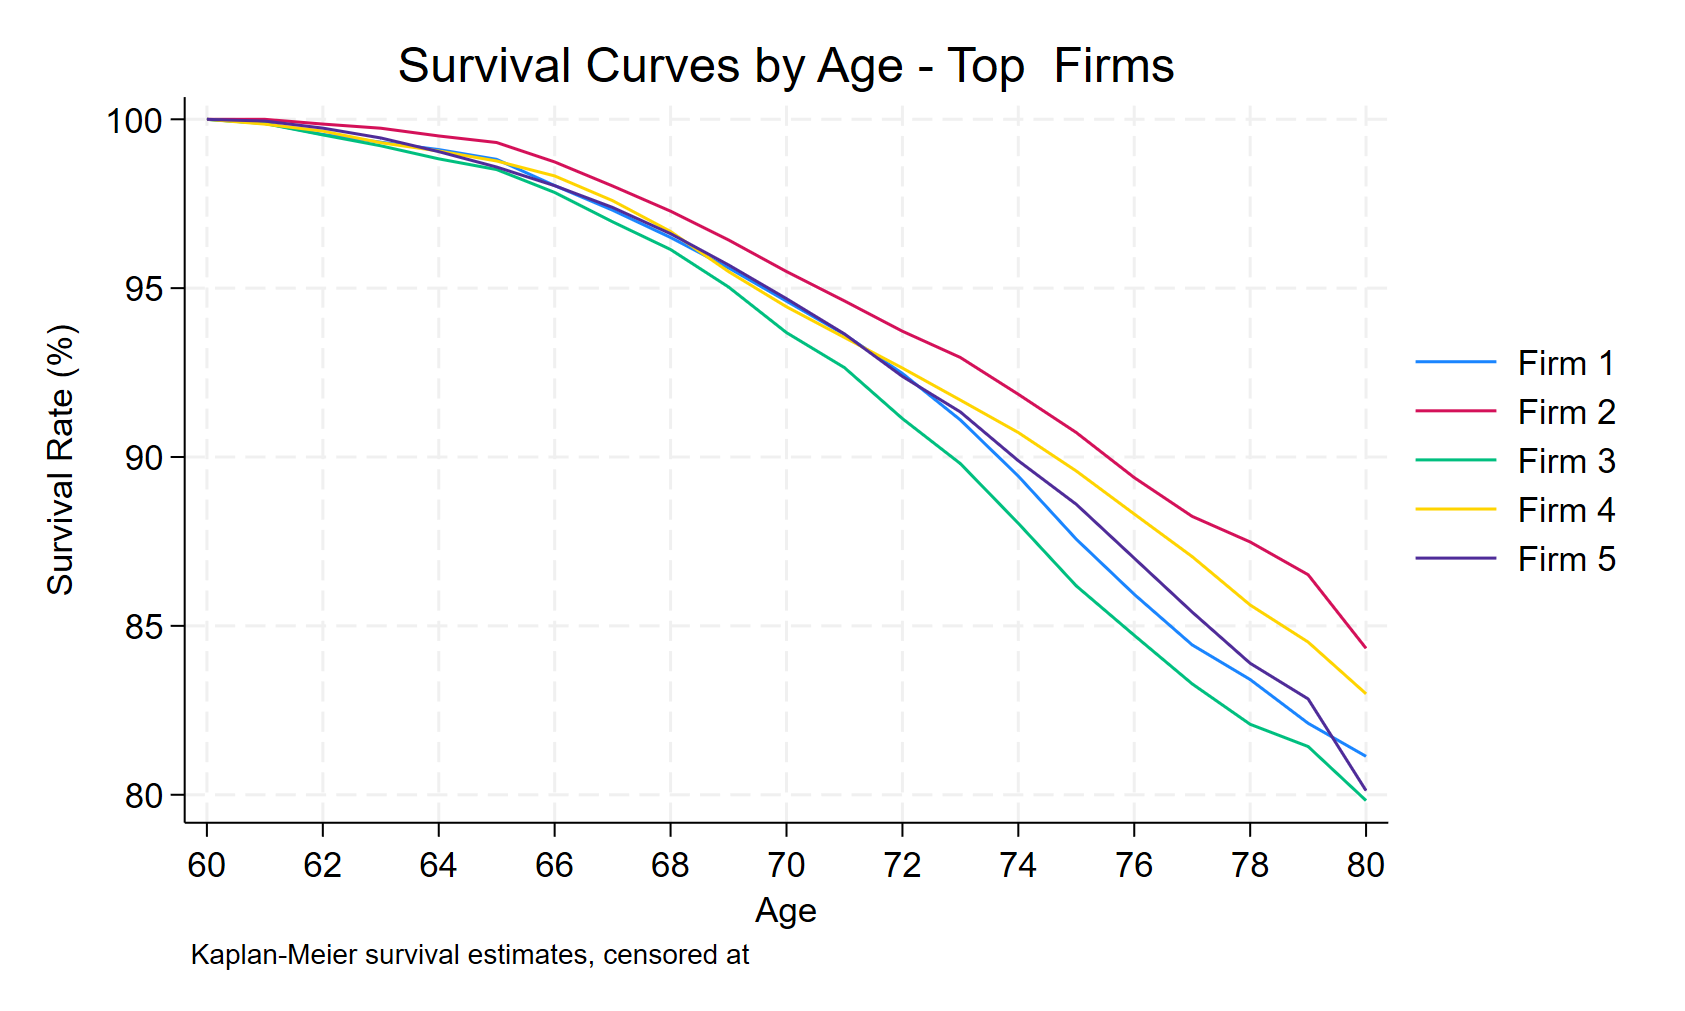
\includegraphics[width=0.6\linewidth]{figures//IE4/IE4_survival_curves_by_age_top_firms.png}
     %\caption{Enter Caption}
     \label{fig:placeholder}
 \end{figure}

\end{frame}
 

\begin{frame}{Frame Title}
Heterogeneity in terms of relying on external offers. 
 \begin{figure}
     \centering
     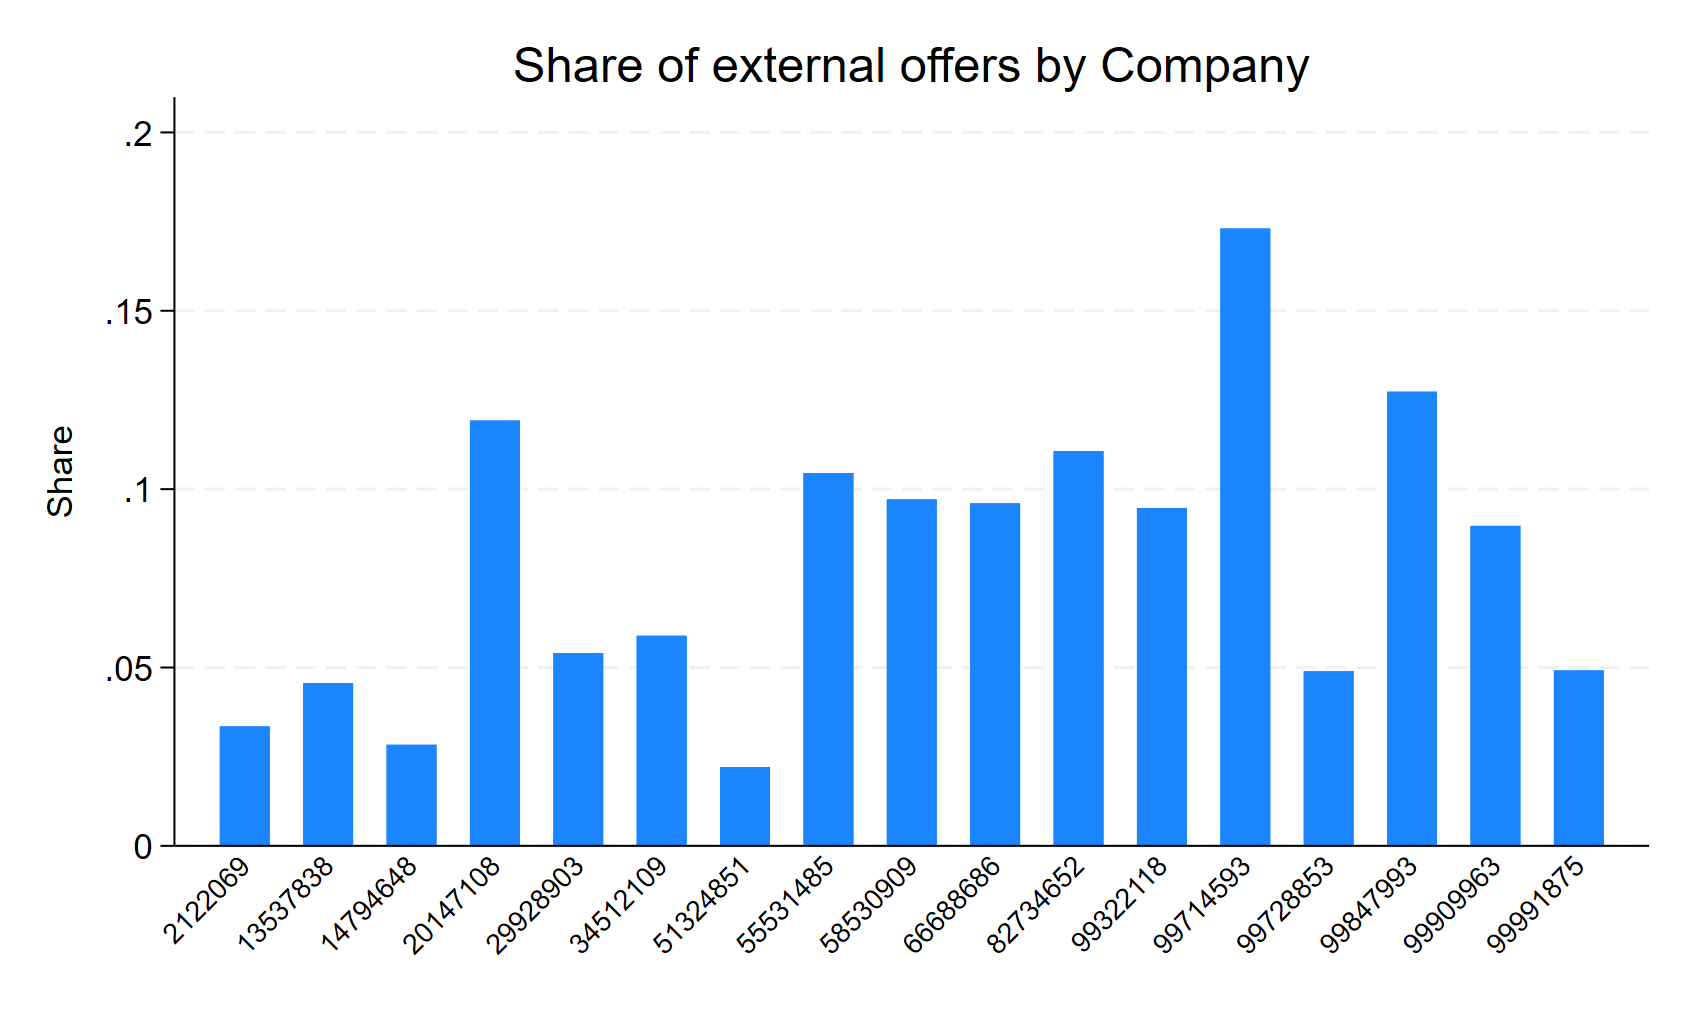
\includegraphics[width=0.6\linewidth]{figures//IE4/IE4_variation_share_external.png}
     %\caption{Enter Caption}
     \label{fig:placeholder}
 \end{figure}
\end{frame}
 

\begin{frame}{Frame Title}
 \begin{figure}
     \centering
     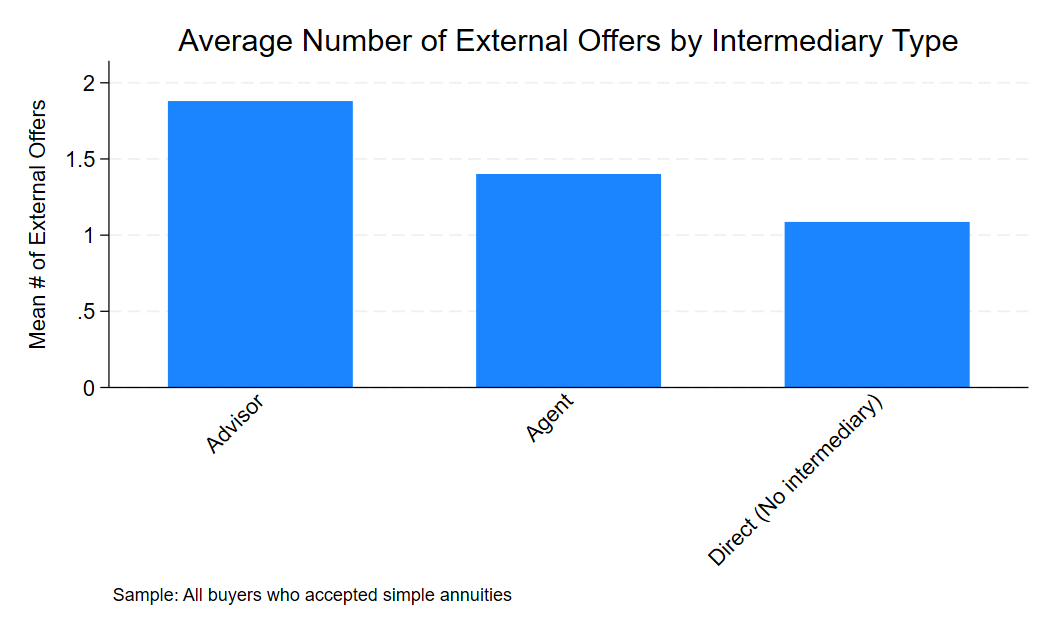
\includegraphics[width=0.6\linewidth]{figures//IE4/IE4_external_offers_by_intermediary.png}
     %\caption{Enter Caption}
     \label{fig:placeholder}
 \end{figure}
\end{frame}



 \begin{frame}{Frame Title}
 \begin{figure}
     \centering
     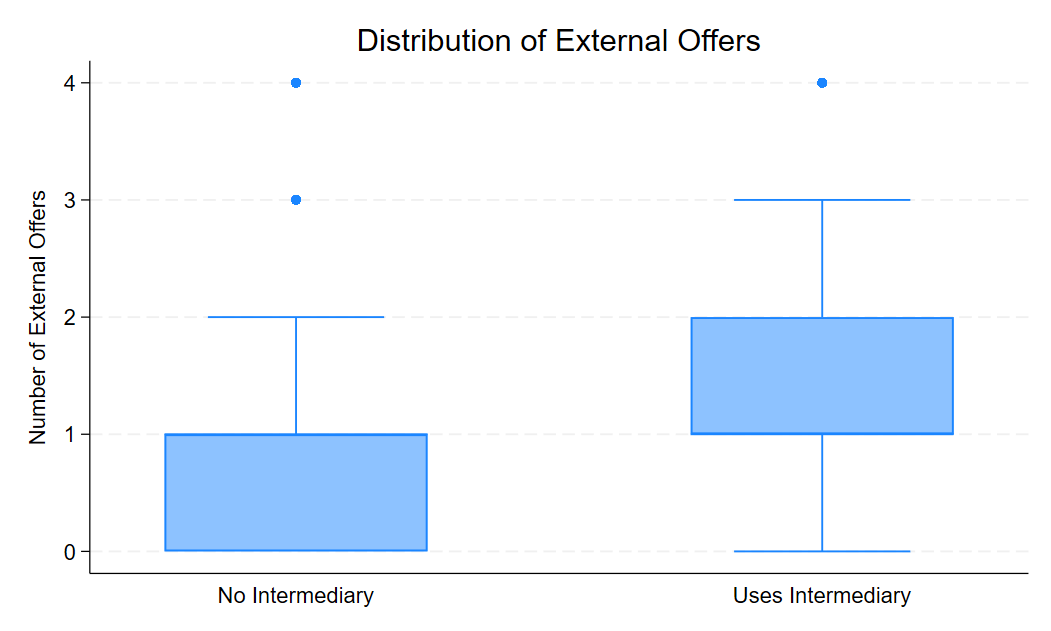
\includegraphics[width=0.6\linewidth]{figures//IE4/IE4_intermediary_search_box.png}
     %\caption{Enter Caption}
     \label{fig:placeholder}
 \end{figure}
\end{frame}


 
 \begin{frame}{Frame Title}
 Intermediaries affect search. 
 \begin{figure}
     \centering
     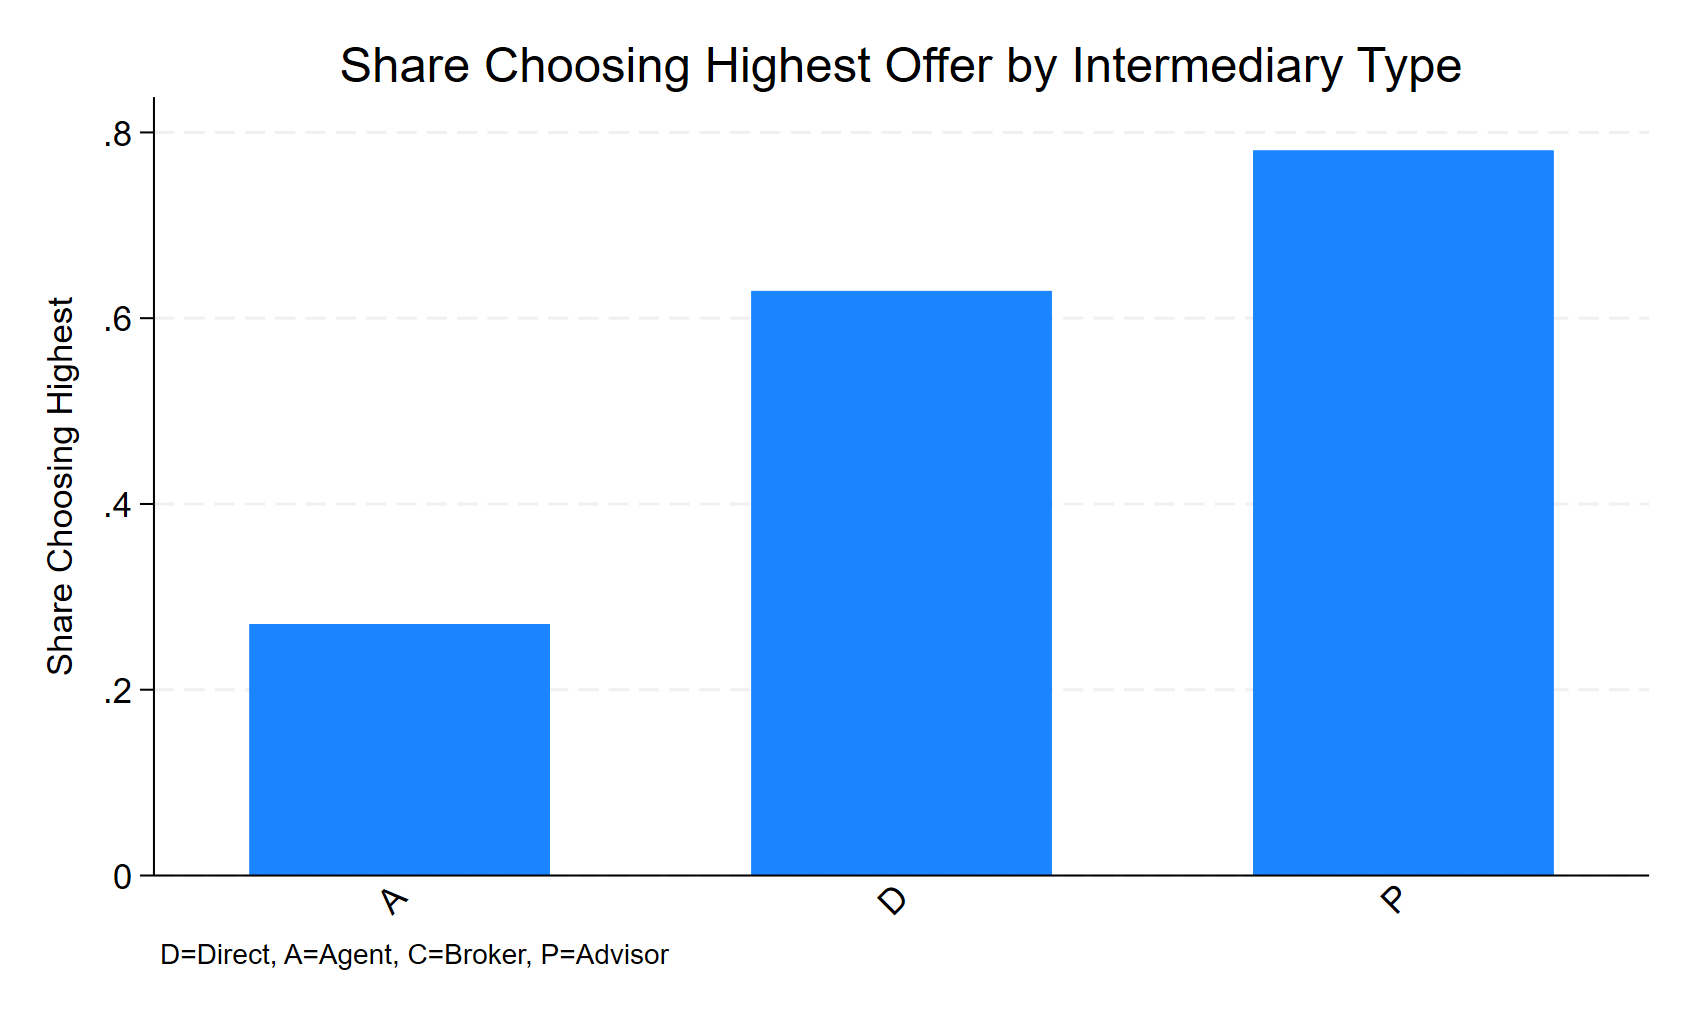
\includegraphics[width=0.6\linewidth]{figures//IE4/IE4_highest_by_intermediary_type.png}
     %\caption{Enter Caption}
     \label{fig:placeholder}
 \end{figure}
\end{frame}


 
\begin{frame}{Frame Title}

\begin{figure}
     \centering
     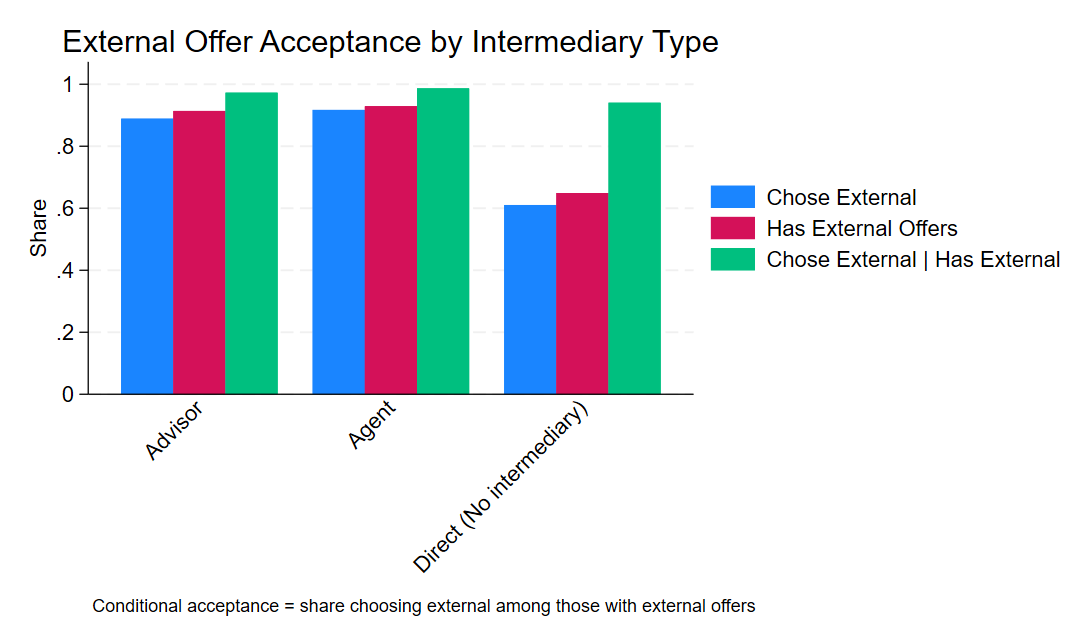
\includegraphics[width=0.6\linewidth]{figures//IE4/IE4_external_acceptance_by_intermediary.png}
     %\caption{Enter Caption}
     \label{fig:placeholder}
 \end{figure}
\end{frame}
 




\end{document}